\chapter{Structure of an Multi-dimensional Array}
The new sparse array have to be compliant with the API and inter-operable with the current dense array implementation.



\section{Storing an Array}
\label{sec:storing}

A dense array is stored as a single contiguous block of memory, flattened in a one-dimensional array. Arrays are stored off-heap (outside the JVM memory management). The reasons behind this design decision are numerous: better performance (avoid the interruptions of the garbage collector), better interoperability with BLAS libraries, and to avoid the disadvantages of the {JVM} such as the limited size of arrays due to the integer indexing (limited to $2^{31}-1 \cong 2.14 \text{ billion}$ elements)

There are two methods to store a multi-dimensional array into a linear memory space: row-major order (C) or column-major order (Fortran). Figure \ref{fig:orders} shows how a two-dimensional array is stored according to the order.

\begin{figure}[h]
	\begin{center}
		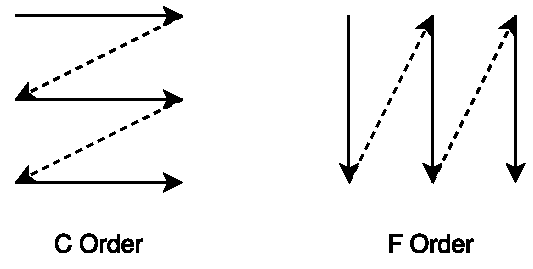
\includegraphics[width=2.5in]{images/c_f_Orders.pdf} 
		\label{fig:cOrders}
	\end{center}
	\[
	A = 
	\begin{bmatrix}
	a_{11} &  a_{12} & a_{13} \\
	a_{21} &  a_{22} & a_{23}
	\end{bmatrix}
	\quad\Rightarrow\quad
	\begin{aligned}
	C-Order = 
	\begin{bmatrix}
	a_{11} &  a_{12} & a_{13} & a_{21} &  a_{22} & a_{23}
	\end{bmatrix}
	\\
	F-Order = 
	\begin{bmatrix}
	a_{11} &  a_{21} & a_{12} & a_{22} &  a_{31} & a_{13}
	\end{bmatrix}
	\end{aligned}
	\]
\caption{Comparison between C-order and F-order}
\label{fig:orders}

\end{figure}

The data is accessed via strides which define how to index a contiguous block of data. For each dimension, it defines by how many values two consecutive elements are separated. In the case of matrix $A$ defined in figure \ref{fig:orders}, the strides would be $(3, 1)$ in case of C-order and $(1, 3)$ in case of F-order. Strides $(3, 1)$ means that each row is separated by 3 values and each column is separated by 1 value.

\subsection{Data Buffer}
The \textit{DataBuffer} is a storage abstraction which provides optimal storage and retrieval depending on the backend. The data is stored off-heap through JavaCPP. It is basically a wrapper around a pointer and an indexer with utility methods to access and modify the data. 
The pointer points to the allocated memory space and the indexes provides an easy-to-use and efficient way to access a multi-dimensional memory space.

The implementation of the \textit{DataBuffer} depends on the data type, because of the length needed to store a single value (int -> 32 bits, long -> 64bits, float -> 32bits, double -> 64bits, assuming a 64bit-architecture).

In the GPU backend, the data is allocated on the host (in the RAM) and on the device (on the GPU), the \textit{DataBuffer} has two pointers instead of one.

\subsection{Parameters of an Array}
The information about the shape of the array are grouped in a \textit{DataBuffer} object called ShapeInformation. It groups these following information:

\begin{description}[leftmargin=!,labelwidth=\widthof{\bfseries ElementWiseStride}]
	\item [Rank] The number of dimension of the array.
	\item [Shape] The shape of the array.
	\item [Strides] Provides information about the logical layout of the array for each dimension.
	\item [Offset] Provides the position of the first value in memory that belongs to the array or view (explained in section \ref{sec:viewsDesc}).
	\item [ElementWiseStride] Indicates how two contiguous elements are physically separated in memory.
	\item[Order] C or F order
\end{description}


\section{Views}
\label{sec:viewsDesc}
The data in memory can be shared by multiple \textit{NDArrays}. An \textit{NDArray} can refer to a subset of another \textit{NDArray}. We say that such an array is a view of the original array. This is a powerful concept that avoid the unnecessary copy of the data which is a very expensive operation.

Since the memory space is shared, changes to array will impact the content of the other arrays. Figure \ref{fig:sharememView} illustrates how a view shares its data with its original array.


\begin{figure}[!h]
	\begin{center}
		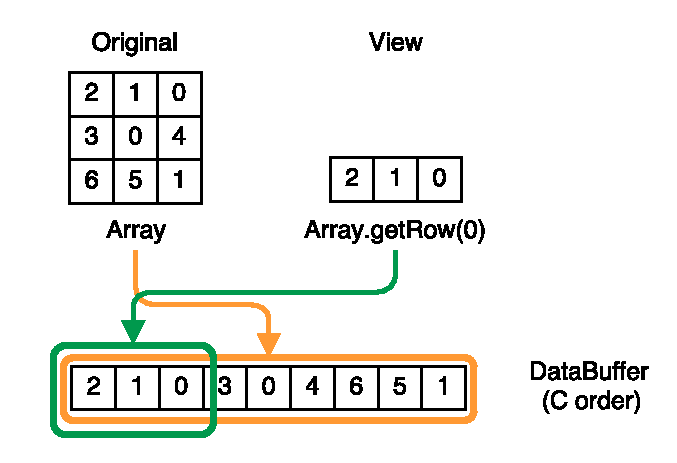
\includegraphics[width=3.5in]{images/views.pdf} 
		\caption{View shares memory with the original array}		
		\label{fig:sharememView}
	\end{center}
\end{figure}


We can also get a part of a view. In this case we have a view of a view and the all share the memory space of the original array. The figure \ref{fig:hierachyview} shows a possible hierarchy of views. The DataBuffer of the views contains a pointer to the original DataBuffer and a pointer the memory space.


\begin{figure}[h]
	\begin{center}
		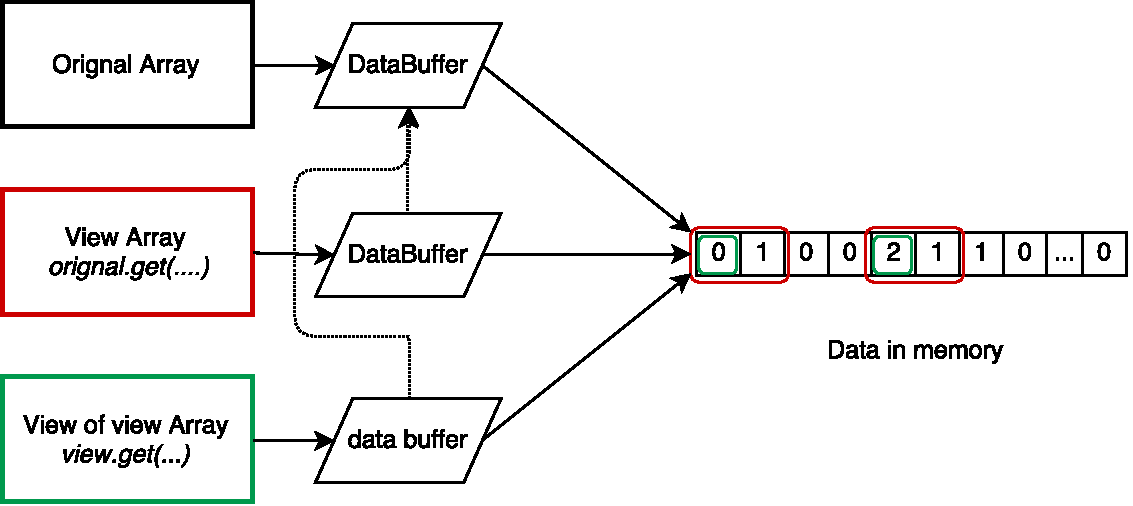
\includegraphics[width=5.5in]{images/hierarchyview.pdf} 
		\caption{View hierarchy}
		\label{fig:hierachyview}
	\end{center}
\end{figure}


\section{Indexes}

\textit{NDArrays} can be accessed through a combination of indexes. There are many way to index an array. For each dimension of the original array, we can specify if we want everything, an interval or a specific value of it. It gives a lot of flexibility to access sub-part of a array. 

Nd4j emulates the  syntax of Numpy\cite{numpy} and use a similar mechanism to indexes the arrays. Among the different indexes we can note the intervals, the points,\dots

Each index implements the interface \textit{INDArrayIndex} and extends from \textit{NDArrayIndex}.

The indexes provide an efficient mechanism to access Tensors along dimension. A tensor along dimension (TAD) is a view of an actual tensor with a lower rank. The TAD are a very powerful concept to perform fast and optimized operations on tensors.

\section{Operations}

Nd4j defines five types of operations:
\begin{enumerate}
\item Scalar: element-wise operations such as addition or multiplication where the same operation is applied on each element of the array. 
\item Transform: in-place operations such as logarithm or cosine. There are usually executed in an element-wise manner but it's not always the case; some can be applied along a dimension.
\item Accumulation: Also called Reduction. Operations applied over the whole ndarray or along a dimension such as the sum of all values.
\item Index Accumulation: Similar to accumulation operations but return an index instead of a value. A classic operation is getting the maximum or minimum value along a dimension.
\item Broadcast: Some of the more useful operations are vector operations, such as \textit{addRowVector} which add a row vector to every row of a matrix.
\end{enumerate}
